\documentclass{article}
\usepackage{tikz}

\begin{document}

\begin{figure}[h]
    \centering
    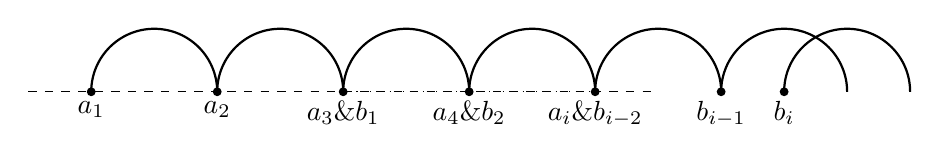
\begin{tikzpicture}[scale=0.8]
        % Draw the horizontal line with labels
        \draw[dashed] (-5,0) -- (5,0);
        
        % Draw the labels for the points on the left side
        \foreach \x/\label in {-4/a_{1}, -2/a_{2}, 0/a_{3}\&b_{1}, 2/a_{4}\&b_{2}} {
            \fill (\x,0) circle (2pt) node[below] {$\label$};
        }
        
        % Draw the labels for the points on the right side
        \foreach \x/\label in {4/a_{i}\&b_{i-2}, 6/b_{i-1}, 7/b_{i}} {
            \fill (\x,0) circle (2pt) node[below] {$\label$};
        }
        
        % Draw the arcs connecting the points
        \draw[thick] (-4,0) arc (180:0:1);
        \draw[thick] (-2,0) arc (180:0:1);
        \draw[thick] (0,0) arc (180:0:1);
        \draw[thick] (2,0) arc (180:0:1);
        \draw[thick] (4,0) arc (180:0:1);
        \draw[thick] (6,0) arc (180:0:1);
        \draw[thick] (7,0) arc (180:0:1);
        
        % Add a dotted line between the middle arcs
        \draw[dotted] (0,0) -- (4,0);
    \end{tikzpicture}
    \caption{The output of \ref{mainint}. $a_3$, $b_1$ have been drawn in the same place because we do not know which is larger.}
    \label{fig:diagram}
\end{figure}

\end{document}